\documentclass[12pt]{article}
\usepackage{cmap}
\usepackage[T2A]{fontenc}
\usepackage[english]{babel}
\usepackage{amsmath,amssymb,amsfonts,amsthm}
\usepackage{enumitem}
\usepackage{csquotes}
\usepackage{graphicx}
\usepackage[margin=2cm]{geometry}
\usepackage{tikz}
\usepackage[titles]{tocloft}
\usepackage{mathrsfs}
\usepackage{array}
\usepackage{longtable}
\usepackage{mathtools}
\usepackage{twemojis}
\usepackage{hyperref}

\hypersetup{colorlinks=true, linkcolor=blue, citecolor=blue}
\usetikzlibrary{math}

\newcommand{\E}{\operatorname{\mathbb{E}}}
\newcommand{\R}{\mathbb{R}}
\newcommand{\N}{\mathbb{N}}
\newcommand{\var}{\operatorname{Var}}
\newcommand{\cov}{\operatorname{Cov}}
\newcommand{\rank}{\operatorname{rank}}
\newcommand{\diag}{\operatorname{diag}}
\newcommand{\im}{\operatorname{im}}
\newcommand{\tr}{\operatorname{trace}}
\newcommand{\I}{\operatorname{\mathbb{I}}}
\renewcommand{\P}{\operatorname{\mathbb{P}}} 

\renewcommand{\qedsymbol}{\twemoji{poop}}

\theoremstyle{remark}
\newtheorem{remark}{Remark}[section]

\newtheorem{claim}{Claim}

\theoremstyle{plain}
\newtheorem{theorem}{Theorem}[section]

\theoremstyle{plain}
\newtheorem{lemma}{Lemma}[section]

\title{Techinical details on the implementation}
\author{}

\begin{document}
\maketitle

\tableofcontents
\newpage

\selectlanguage{english}
\newpage
\section{Theory}
\begin{figure}[htpb!]
    \centering
    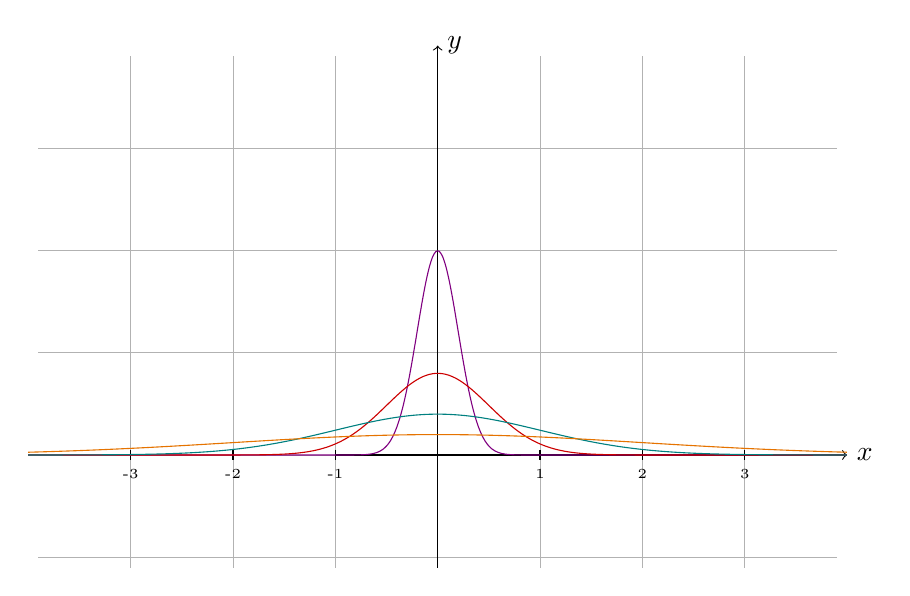
\begin{tikzpicture}[scale=1.3]
        \tikzmath{\m = 0;}
        \draw[->]  (-1,0) -- (4,0) node[right] {$x$};
        \draw[->]  (0,-1.1) -- (0,4) node[right] {$y$};
        \draw[very thin, opacity=0.3] (-3.9,-1.1) grid (3.9,3.9);
        
        \foreach \x in {-3,-2,-1,1,2,3}
        \draw (\x, 0.05) -- (\x, -0.05) node[below, font=\tiny] {\x};
        
        \foreach \sgm/\col in {0.2/violet, 0.5/red!80!black, 1/teal, 2/orange!90!black}
            {    
                \draw[domain=-4:4, samples=250, smooth, \col]
                plot (\x, {1/(\sgm*sqrt(2*pi))*exp(-((\x-\m)*(\x-\m))/(2*\sgm*\sgm))});
            }
    \end{tikzpicture}
    \caption{Normal PDF $\frac{1}{\sqrt{2\pi}\sigma}e^{-\frac{(x-\mu)^2}{2\sigma^2}}$}
\end{figure}

\subsection{Central limit theorem}
For $X_1, ..., X_n \overset{iid}{\sim} X$ we have:
\[\frac{\sum_{i=1}^{n} X_i - n\E[X]}{\sqrt{n\var(X)}} \overset{d}{\rightarrow} \mathcal{N}(0, 1)\]
meaning the CDF of the normalized empirical mean converges to the CDF of the standard normal distribution. Using this theorem we run the approximation using the binomial distribution with $p = 0.3$ and $n = 1000$. Figure \ref{fig:cdf qq} illustrates the approximation result.

\begin{figure}[htpb!]
    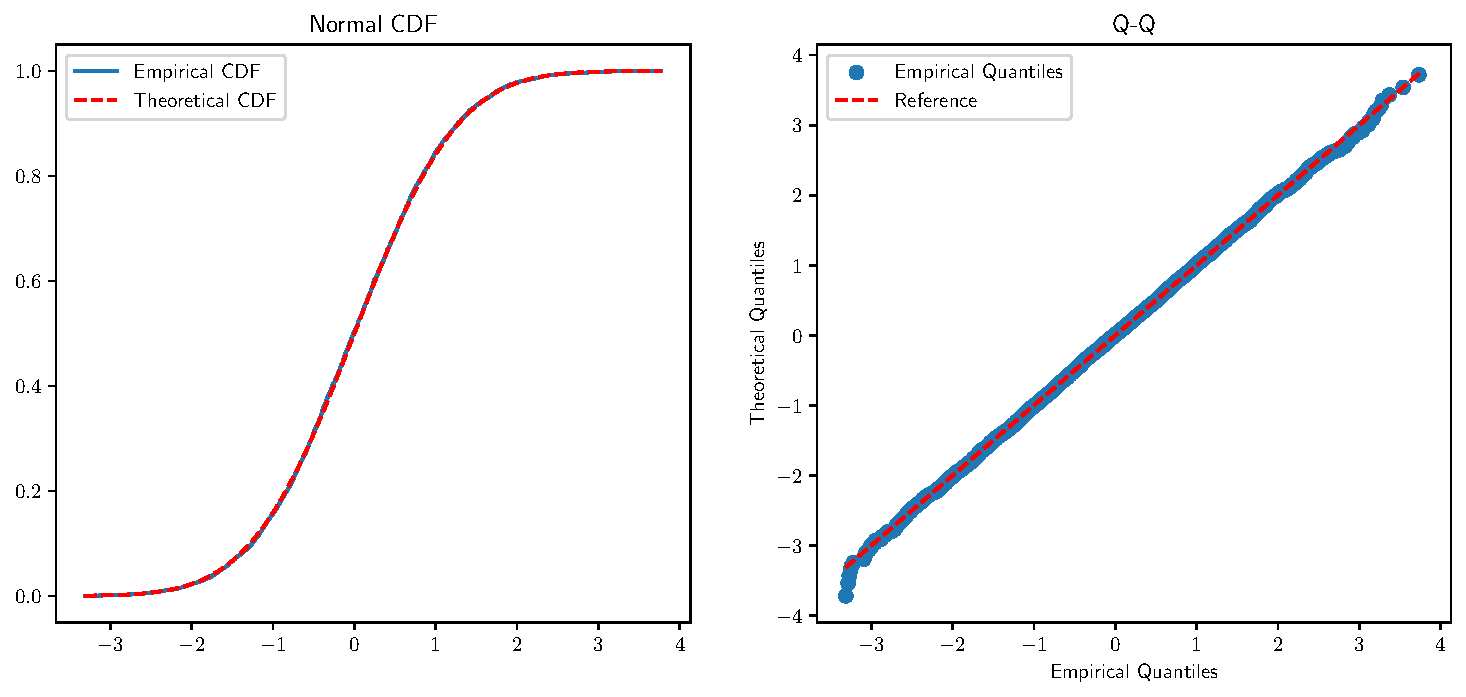
\includegraphics[width = \textwidth]{cdf_qq.pdf}
    \caption{CDF and Q-Q plot}
    \label{fig:cdf qq}
\end{figure}

\subsection{Approximation quality}
We want to estimate how accurate is the estimate:
\[F_n(t)
    = \frac{1}{n} \sum_{i=1}^{n} \I_{X_i \leq t}
    = \frac{1}{n} \sum_{i=1}^{n} \I_{(-\infty,t]}(X_i)\]

The estimate is unbiased since:
\begin{equation} \label{eq:unbiasedness}
    \begin{split}    
        \E \left[\frac{1}{n} \sum_{i=1}^{n} \I_{X_i \leq t}\right]
        = \frac{1}{n} \sum_{i=1}^{n} \E \left[\I_{X_i \leq t}\right]
         & \overset{*}{=} \frac{1}{n} \sum_{i=1}^{n} \P (X_i \leq t)
        \\ &\overset{**}{=} \frac{1}{n} \sum_{i=1}^{n} \P (X \leq t)
        = \P (X \leq t)
    \end{split}
\end{equation}
where $*$ holds since as we integrate the indicator function we get the probability of the event, and $**$ holds since $X_i \sim X$.

Each $\I_{X_i \leq t}$ is bounded by $[0, 1]$, so we can use Hoeffding's inequality to get a bound on the probability of the estimate being far from the true value:
\begin{equation} \label{eq:hoeffding bound}
    \P \left(\left|\frac{1}{n} \sum_{i=1}^{n} \I_{X_i \leq t} - \P (X \leq t)\right| \geq \delta\right)
    = \P \left(\left|\frac{1}{n} \sum_{i=1}^{n} \I_{X_i \leq t} - F(t)\right| \geq \delta\right)
    \leq 2 e^{-2 n \delta^2}
\end{equation}

Figure~\ref{fig:hoeffding} illustrates the bound for different values of $\delta$.
\begin{figure}[htpb!]
    \centering
    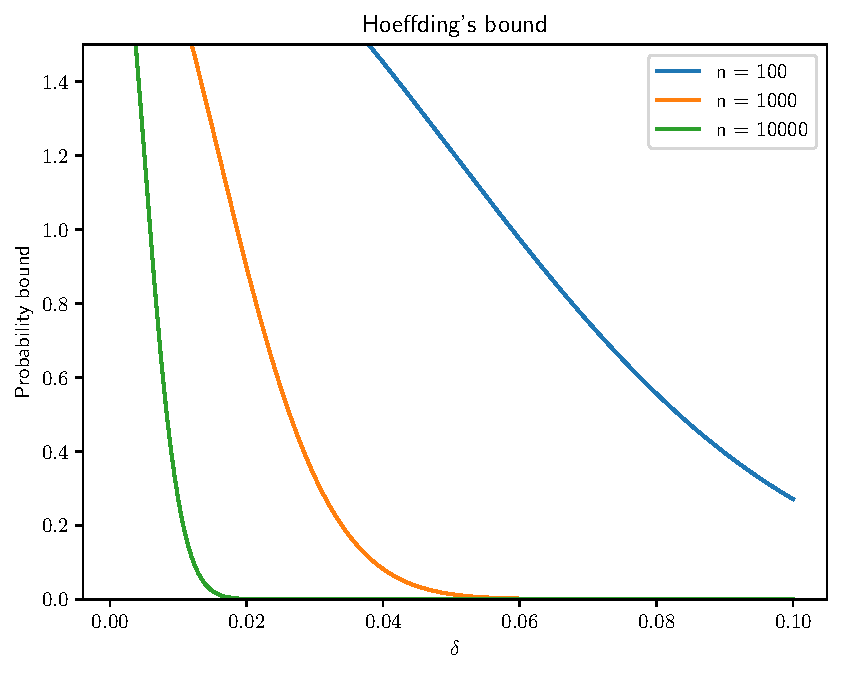
\includegraphics[width = 0.7\textwidth]{hoeffding.pdf}
    \caption{Hoeffding's inequality bound}
    \label{fig:hoeffding}
\end{figure}

For the almost sure convergence refer to \href{https://en.wikipedia.org/wiki/Glivenko%E2%80%93Cantelli_theorem}{Glivenko---Cantelli theorem}, which states the following:
\begin{theorem}[Glivenko---Cantelli theorem] \label{thm:glivenko-cantelli}
    Let $X_1, X_2, ... \overset{iid}{\sim} X$ and $F(x)$ be CDF of $X$. Moreover let $F$ be continuous. Then we have:
    \[\P \left(\sup_{t \in \R} \left|F_n(t) - F(t) \right| \to 0 \right) = 1\]
    where
    \[F_n(t) = \frac{1}{n} \sum_{i=1}^{n} \I_{(-\infty,t]}(X_i)\]
\end{theorem}

\begin{proof}[Proof of Theorem~\ref{thm:glivenko-cantelli}]
    Fix $-\infty = x_0 \leq x_1 \leq ... \leq x_m = \infty$, s.t. $F(x_k) + 1/m = F(x_{k + 1})$ (using intermediate value theorem assuming $F$ is continuous) for all $k \in \{0, ..., m - 1\}$. Then if $x \in [x_{k-1}, x_k]$ by monotonicity of $F_n$ and $F$ we have:
    \begin{itemize}    
        \item $F_n(x) - F(x)
                  \geq F_n(x_{k-1}) - F(x_{k})
                  = F_n(x_{k-1}) - F(x_{k-1}) - 1/m$
        \item $F_n(x) - F(x)
                  \leq F_n(x_{k}) - F(x_{k - 1})
                  = F_n(x_{k}) - F(x_{k}) + 1/m$
    \end{itemize}
    
    Thus we have that for each $x \in \R$ there exists $k \in \{1, ..., m\}$ s.t. $x \in [x_{k-1}, x_k]$ hence:
    \begin{equation} \label{eq:epsilon boundedness}
        \begin{split}    
            \sup_{x \in \R} |F_n(x) - F(x)| \leq \max_{k \in \{0, ..., m\}} |F_n(x_{k}) - F(x_{k})| + 1/m
        \end{split}
    \end{equation}
    
    If we now suppose that for some $\omega \in \Omega$:
    \[\sup_{x \in \R} |F_n(x)(\omega) - F(x)| > \varepsilon + 1/m\]
    then by \eqref{eq:epsilon boundedness} we have that:
    \[\max_{k \in \{0, ..., m\}} |F_n(x_{k})(\omega) - F(x_{k})| > \varepsilon\]
    thus:
    \begin{equation} \label{eq:probability monotonicity}
        \P\left(\sup_{x \in \R} |F_n(x) - F(x)| > \varepsilon + 1/m \text{ i.o.} \right)
        \leq \P\left(\max_{k \in \{0, ..., m\}} |F_n(x_{k}) - F(x_{k})| > \varepsilon \text{ i.o.} \right)
    \end{equation}
    as $\forall n \in \N$ for which the left hand side event occurs the right hand side event event occurs as well.
    
    Since $F_n(t)$ is the sum of $n$ independent random variables, we can use the strong law of large numbers (the estimate is unbiased \eqref{eq:unbiasedness}, $\I_{(-\infty,t]}(X_i)$ are independent) to get that for each $k \in \{0, ..., m\}$:
    \[\P \left(\lim_{n \to \infty} F_n(x_k) = F(x_k)\right) = 1\]
    
    Thus for each $\varepsilon > 0$ we have:
    \[\P \left(|F_n(x_k) - F(x_k)| > \varepsilon \text{ i.o.}\right) = 0\]
    and by union bound we get:
    \[\P \left(\bigcup_{k=0}^{m} \{|F_n(x_k) - F(x_k)| > \varepsilon \text{ i.o.}\}\right)
        \leq \sum_{k=0}^{m} \P \left(|F_n(x_k) - F(x_k)| > \varepsilon \text{ i.o.}\right) = 0\]
    
    \begin{claim} \label{cl:limsup commutativity}
        Let ${(A_n)}_{n \in \N}, {(B_n)}_{n \in \N} \in \mathcal{F}$ be two sequences of events. Then we have:
        \[\limsup_{n \to \infty} (A_n \cup B_n)
            = \limsup_{n \to \infty} A_n \cup \limsup_{n \to \infty} B_n\]
    \end{claim}
    \begin{proof}[Proof of Claim~\ref{cl:limsup commutativity}]
        \[\limsup_{n \to \infty} (A_n \cup B_n)
            = \bigcap_{n=1}^{\infty} \bigcup_{m=n}^{\infty} (A_m \cup B_m)
            \overset{*}{=} \bigcap_{n=1}^{\infty} \left(\left(\bigcup_{m=n}^{\infty} A_m\right) \cup \left(\bigcup_{m=n}^{\infty} B_m\right) \right)\]
        where $*$ holds by associativity and commutativity of union.
        
        Denote:
        \[\tilde{A}_n = \bigcup_{m=n}^{\infty} A_m \quad \tilde{B}_n = \bigcup_{m=n}^{\infty} B_m\]
        
        We have that $\tilde{A}_n$ and $\tilde{B}_n$ are decreasing sequences of events.
        
        \begin{enumerate}[align=left]
            \item[``$\subset$''] Suppose:
                  \[\omega \in \bigcap_{n=1}^{\infty} (\tilde{A}_n \cup \tilde{B}_n)
                      \Rightarrow \omega \in \tilde{A}_n \cup \tilde{B}_n \; \forall n \in \N\]
                  meaning for each $n \in \N$ $\omega \in \tilde{A}_n$ or $\omega \in \tilde{B}_n$. Assume that for some $k \in \N$ $\omega \notin \tilde{A}_k$. Then for any $n > k$ we have that $\omega \notin \tilde{A}_n$, so we must have $\omega \in \tilde{B}_n$ for all $n > k$. Since $\tilde{B}_n$ is decreasing:
                  \[\omega \in \bigcap_{n = k}^{\infty} \tilde{B}_n = \bigcap_{n = 1}^{\infty} \tilde{B}_n\]
                  
                  Otherwise if $\omega \in \tilde{A}_n$ for all $n \in \N$ we have:
                  \[\omega \in \bigcap_{n = 1}^{\infty} \tilde{A}_n\]
                  which implies:
                  \[\omega \in \left(\bigcap_{n = 1}^{\infty} \tilde{A}_n \right) \cup \left(\bigcap_{n = 1}^{\infty} \tilde{B}_n \right)\]
            \item[``$\supset$''] Suppose:
                  \[\omega \in \left(\bigcap_{n = 1}^{\infty} \tilde{A}_n \right) \cup \left(\bigcap_{n = 1}^{\infty} \tilde{B}_n \right)\]
                  which means either $\omega \in \bigcap_{n = 1}^{\infty} \tilde{A}_n$ or $\omega \in \bigcap_{n = 1}^{\infty} \tilde{B}_n$. In the first case we have that $\omega \in \tilde{A}_n$ for all $n \in \N$, which implies $\omega \in \tilde{A}_n \cup \tilde{B}_n$ for all $n \in \N$. The second case is analogous.
        \end{enumerate}
    \end{proof}
    
    With the Claim~\ref{cl:limsup commutativity} we can rewrite the union of events as:
    \begin{align}    
        \left\{\max_{k \in \{0, ..., m\}} |F_n(x_k) - F(x_k)| > \varepsilon \text{ i.o.} \right\}
         & = \left\{\left(\bigcup_{k \in \{0, ..., m\}} |F_n(x_k) - F(x_k)| > \varepsilon \right) \text{ i.o.}\right\} \notag
        \\ &= \left\{\bigcup_{k \in \{0, ..., m\}} \left(|F_n(x_k) - F(x_k)| > \varepsilon \text{ i.o.} \right)\right\} \label{eq:infinitely often bounded}
    \end{align}
    
    Equation~\ref{eq:probability monotonicity} together with equation~\ref{eq:infinitely often bounded} gives us:
    \[\P \left(\sup_{x \in \R}|F_n(x) - F(x)| > \varepsilon + 1/m \text{ i.o.}\right) = 0\]
    
    Finally since $m$ is arbitrary we can choose $m \geq 2 / \tilde{\varepsilon}$ and $\varepsilon = \tilde{\varepsilon} / 2$ to get:
    \[\P \left(\sup_{x \in \R}|F_n(x) - F(x)| > \tilde{\varepsilon} \text{ i.o.}\right) = 0 \quad \forall \tilde{\varepsilon} > 0\]
    which is equivalent to:
    \[\P \left(\sup_{x \in \R}|F_n(x) - F(x)| \to 0\right) = 1\]
\end{proof}

\begin{remark}    
    The proof translates bounding an uncountable set of points to bounding a finite set of points. This result is of interest since it shows uniform convergence of the empirical CDF including the tails of the distribution, which is important for statistical inference.
\end{remark}

\begin{theorem}[Rate of convergence] \label{thm:rate of convergence}
    Let $X_1, X_2, ... \overset{iid}{\sim} X$ and $F(x)$ be CDF of $X$. Moreover let $F$ be continuous. Then we have:
    \[\P \left(\sup_{t \in \R} \left|F_n(t) - F(t) \right| \geq \delta\right)
        \leq 4\left(1 + \frac{1}{\delta}\right)e^{-\frac{n\delta^2}{2}}, \quad \forall \delta > 0\]
    where
    \[F_n(t) = \frac{1}{n} \sum_{i=1}^{n} \I_{(-\infty,t]}(X_i)\]
\end{theorem}
\begin{proof}[Proof of Theorem~\ref{thm:rate of convergence}]
    Choose the points $x_0, ..., x_m$ as in the proof of Theorem~\ref{thm:glivenko-cantelli}. Then using the bound \eqref{eq:hoeffding bound} we have:
    \[\P \left(\left|\frac{1}{n} \sum_{i=1}^{n} \I_{X_i \leq t} - F(t)\right| \geq \varepsilon\right)
        = \P \left(\left|F_n(t) - F(t)\right| \geq \varepsilon\right)
        \leq 2e^{-2 n \varepsilon^2}\]
    for all $t \in \R$ including the points $x_0, ..., x_m$. Then using the union bound we have:
    \[\P \left(\max_{k \in \{0, ..., m\}} \left|F_n(x_k) - F(x_k)\right| \geq \varepsilon\right)
        \leq 2(m+1)e^{-2 n \varepsilon^2}\]
    
    Similarly to equation~\ref{eq:probability monotonicity} we have that:
    \begin{align*}    
        \P & \left(\sup_{x \in \R} \left|F_n(x) - F(x)\right| \geq \varepsilon + 1/m\right)
        \\ &\leq \P \left(\max_{k \in \{0, ..., m\}} \left|F_n(x_k) - F(x_k)\right| \geq \varepsilon\right)
        \leq 2(m+1)e^{-2 n \varepsilon^2}
    \end{align*}
    which holds for any $m \in \N$.
    
    Now fix $\delta > 0$, choose $m = \lceil 2/\delta \rceil$, and substitute $\varepsilon = \delta/2$ into the inequality above:
    \[\P \left(\sup_{x \in \R} \left|F_n(x) - F(x)\right| \geq \frac{\delta}{2} + \frac{1}{m}\right)
        \leq 2(m + 1)e^{-\frac{n\delta^2}{2}}\]
    
    Since $m = \lceil 2/\delta \rceil$, we have $1/m \leq \delta/2$, hence:
    \[\left\{\sup_{x \in \R} \left|F_n(x) - F(x)\right| \geq \delta\right\}
        \subseteq \left\{\sup_{x \in \R} \left|F_n(x) - F(x)\right| \geq \frac{\delta}{2} + \frac{1}{m}\right\}\]
    and therefore:
    \[\P \left(\sup_{x \in \R} \left|F_n(x) - F(x)\right| \geq \delta\right)
        \leq 2(m + 1)e^{-\frac{n\delta^2}{2}}\]
    
    Finally, using $m = \lceil 2/\delta \rceil \leq 2/\delta + 1$, we get:
    \[2(m + 1) \leq 2\left(\frac{2}{\delta} + 2\right) = 4\left(1 + \frac{1}{\delta}\right)\]
    so:
    \[\P \left(\sup_{x \in \R} \left|F_n(x) - F(x)\right| \geq \delta\right)
        \leq 4\left(1 + \frac{1}{\delta}\right)e^{-\frac{n\delta^2}{2}}\]
\end{proof}

\begin{figure}[htpb!]
    \centering
    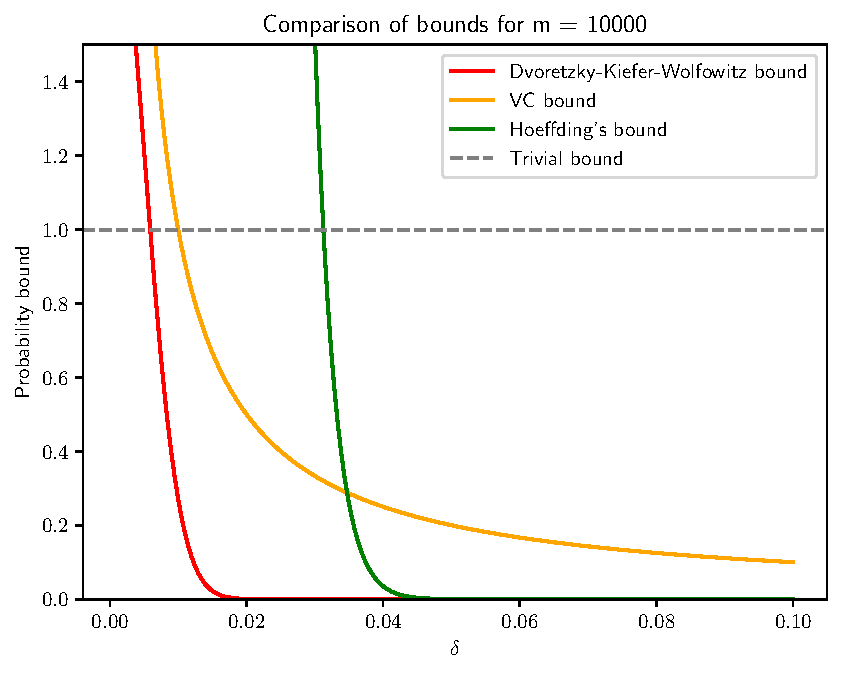
\includegraphics[width = 0.7\textwidth]{bounds_comparison.pdf}
    \caption{\centering Bounds comparison: Hoeffding's inequality (Theorem~\ref{thm:rate of convergence}), Dvoretzky---Kiefer---Wolfowitz inequality (Remark~\ref{rem:dkw}), VC theory bound (Remark~\ref{rem:vc bound})}
    \label{fig:bounds comparison}    
\end{figure}

\begin{remark} \label{rem:dkw}
    For the tighter bound refer to \href{https://en.wikipedia.org/wiki/Dvoretzky%E2%80%93Kiefer%E2%80%93Wolfowitz_inequality}{Dvoretzky---Kiefer---Wolfowitz inequality}, which states the following:
    \[\P \left(\sup_{t \in \R} \left|F_n(t) - F(t) \right| \geq \delta\right)
        \leq 2e^{-2n\delta^2}, \quad \forall \delta \geq 0\]
    
    Note that this is the same exact bound as in \eqref{eq:hoeffding bound} but uniform over all $t \in \R$
\end{remark}

\newcommand{\loss}{\operatorname{\mathscr{L}}}
\begin{remark} \label{rem:vc bound}
    By VC theory we have that the hypothesis class:
    \[\mathcal{H} = \{h_t = \I_{(-\infty, t]}: t \in \R\}\]
    has VC dimension $d = 1$. Note that for the distribution $\mathcal{D}$ induced by $(X, 0)$, where $X$ is a random variable and $0$ is the label, we have that the training loss for the sample $\mathcal{T} = ((X_1, 0), ..., (X_n, 0)) \overset{iid}{\sim} \mathcal{D}$ is given by:
    \[\loss_{\mathcal{T}} = \frac{1}{n} \sum_{i=1}^{n} \ell_{0-1}(\I_{(-\infty, t]}(X_i), 0)
        = \frac{1}{n} \sum_{i=1}^{n} \I_{(-\infty, t]}(X_i)
        = F_n(t)\]
    
    The true loss is given by:
    \[\loss_{\mathcal{D}}(h_t) 
        = \E_{(X, 0) \sim \mathcal{D}}[\ell_{0-1}(\I_{(-\infty, t]}(X), 0)]
        = \E_{X \sim \mathcal{D}}[\I_{(-\infty, t]}(X)]
        = \P(X \leq t)
        = F(t)\]
    
    By Fundamental Theorem of Statistical Learning Theory for any distribution $\mathcal{D}$:
    \[\E \left[\sup_{h \in \mathcal{H}} \left|\loss_{\mathcal{T}}(h) - \loss_{\mathcal{D}}(h) \right| \right]
        = \E \left[\sup_{t \in \R} |F_n(t) - F(t)| \right]
        \leq C\sqrt{\frac{\mathrm{VC}(\mathcal{H})}{n}}\]
    for some constant $C > 0$.
    
    By Markov's inequality we have that for any $\delta > 0$:
    \[\P \left(\sup_{t \in \R} |F_n(t) - F(t)| \geq \delta\right)
        \leq \frac{\E\left[\sup_{t \in \R} |F_n(t) - F(t)| \right]}{\delta}
        \leq \frac{C\sqrt{\frac{\mathrm{VC}(\mathcal{H})}{n}}}{\delta}
        = C\sqrt{\frac{1}{n\delta^2}}\]
\end{remark}

\newpage
\section{Linear regression} \label{sec:linear_regression}
Assume the following construction:
\[y_i = \beta^T x_i + \varepsilon_i, \quad \varepsilon_1, ..., \varepsilon_n \overset{iid.}{\sim} \mathcal{N}(0, \sigma^2)\]
where $x_i \in \R^d$ and $\beta \in \R^d$ are fixed

\subsection{Preliminaries}
\begin{lemma}                                                                      
    Let $X: \Omega \to \R^d$ be a random variable and $A \in \R^{d \times d}, b \in \R^d$. Assume that the second moments exist, i.e. $\E [X_i^2] < \infty$ and the covariance matrix is given by $\Sigma$. Then the following properties hold:
    \begin{enumerate}[label=Property \thelemma.\arabic*, align=left]
        \item \label{prop:expectation linearity} $\mathbb{E}[AX + b] = A \cdot \mathbb{E}[X] + b$
        \item \label{prop:covariance linearity} $\cov (AX) = A \cdot \Sigma \cdot A^T$
    \end{enumerate}
\end{lemma}
\begin{remark}                                                    
    Using the fact that the second moment exists and by Jensen's inequality, we have that $\E[X_i] < \infty$ and $\E[X_i^2] < \infty$ for all $i = 1, ..., d$. Therefore the covariance matrix is well-defined, since $\left(\E [|X_i X_j|]\right)^2 = (\E [|X_i| |X_j|])^2 \leq \E [|X_i|^2] \E [|X_j|^2] < \infty$ by Cauchy-Schwarz inequality.
\end{remark}
\begin{proof} \hfill  
    \begin{enumerate}                                                                                                                                        
        \item Trivial
        \item Suppose that the expected value of $X$ is the zero vector. By \ref{prop:expectation linearity} we also have that $\E[AX] = A \E[X] = 0$. Then we have that:
              \begin{align*}                                                                                                                                            
                  \cov((AX)_i, (AX)_j)
                   & = \cov \left(\sum_{k=1}^{d} A_{ik} X_k, \sum_{l=1}^{d} A_{jl} X_l\right)
                  = \E \left(\left(\sum_{k=1}^{d} A_{ik} X_k\right)\left(\sum_{l=1}^{d} A_{jl} X_l\right) \right)
                  \\ & = \E \left[\sum_{k=1}^{d} \sum_{l=1}^{d} A_{ik} X_k X_l A^T_{lj} \right]
                  = \sum_{k=1}^{d} \sum_{l=1}^{d} A_{ik} \E [X_k X_l] A^T_{lj}
                  \\ & = \sum_{k=1}^{d} A_{ik} \left(\sum_{l=1}^{d} \Sigma_{kl} A^T_{lj} \right)
                  = \sum_{k=1}^{d} A_{ik} (\Sigma A^T)_{kj}
                  = (A \Sigma A^T)_{ij}
              \end{align*}
              
              If the expected value of $X$ is not the zero vector, we can define a new random variable $Y = X - \E[X]$, which has the expected value of zero. Then we have that:
              \[\cov (Y_i, Y_j)
                  = \E [Y_i Y_j]
                  = \E[(X_i - \E[X]_i)(X_j - \E[X]_j)]
                  = \cov (X_i, X_j)\]
              Therefore we have that:
              \begin{align*}                                                                                                                                    
                  \cov((AX)_i, (AX)_j)
                   & = \E[(AX - \E[AX])_i \cdot (AX - \E[AX])_j]
                  \\ &\overset{*}{=} \E[(A(X - \E[X]))_i \cdot (A(X - \E[X]))_j]
                  \\ &= \E[(AY)_i \cdot (AY)_j]
                  = \cov((AY)_i, (AY)_j) 
                  \\ &= (A \cov(Y) A^T)_{ij} 
                  = (A \cov(X) A^T)_{ij}
              \end{align*}
              where $*$ follows from \ref{prop:expectation linearity}.
    \end{enumerate}
\end{proof} 

\begin{lemma}[Multivariate normal distribution] \label{lem:multinormal}
    We say that $X: \Omega \to \R^d$ is multivariately normally distributed if and only if there exists a matrix $A \in \R^{d \times d}$ and a vector $b \in \R^d$ such that $X = A Z + b$, where $Z_1, ..., Z_d \overset{iid.}{\sim} \mathcal{N}(0, 1)$.
    
    We have that multivariate normal distribution is closed under linear transformations, i.e. if $X \sim \mathcal{N}(\mu, \Sigma)$ and $Y = AX + b$, then $Y \sim \mathcal{N}(A\mu + b, A \Sigma A^T)$. (For the expectation and covariance refer to \ref{prop:expectation linearity} and \ref{prop:covariance linearity}).
\end{lemma}
\begin{lemma} \label{lem:multivariate independence}
    For the multivariate normal distribution, we have that the components are independent if and only if they are uncorrelated, i.e. $\cov(X_i, X_j) = 0$ for all $i \neq j$.
\end{lemma}

\begin{lemma} \label{lem:projection properties}
    Let $X \in \R^{n \times d}$ be a matrix of full rank, where $n > d$. Define $H = X (X^TX)^{-1}X^T \in \R^{n \times n}$ and $E = \diag \{\underbrace{1, ..., 1}_{n - d}, \underbrace{0, ..., 0}_{d}\}$, then:
    \begin{enumerate}[label=Property \thelemma.\arabic*, align=left]
        \item \label{prop:idempotent symmetric} $I - H$ is symmetric and idempotent.
        \item \label{prop:rank} $\rank(I - H) = n - d$
        \item \label{prop:identity} There exists a matrix $Q$ such that $I - H = Q^T E Q$
        \item \label{prop:kernel image} $\ker (I - H) = \im (X)$
    \end{enumerate}
\end{lemma}
\begin{proof} \hfill 
    \begin{enumerate}                                                                                                                    
        \item This follows by the direct computation:
              \[(I - H)^T 
                  = I - H^T 
                  = I - (X (X^TX)^{-1}X^T)^T
                  = I - (X^T)^T \left((X^TX)^T\right)^{-1} X^T
                  = I - H\]
              \begin{align*}                                                     
                  (I - H)(I - H)
                   & = (I - X (X^TX)^{-1}X^T)(I - X (X^TX)^{-1}X^T)
                  \\ & = I - 2 X (X^TX)^{-1}X^T + X (X^TX)^{-1}X^T X (X^TX)^{-1}X^T
                  \\ & = I - 2 X (X^TX)^{-1}X^T + X (X^TX)^{-1} X^T                 
                  \\ & = I - X (X^TX)^{-1}X^T
                  = I - H
              \end{align*}
        \item Since $I - H$ is idempotent we have that its trace is equal to its rank. Therefore we have that:
              \[\tr(H) 
                  = \tr(X (X^TX)^{-1}X^T)
                  \overset{*}{=} \tr((X^TX)^{-1} X^T X)
                  = \tr(I_d)
                  = d\]
              where $*$ follows from the cyclic property of the trace. Therefore we have that:
              \[\rank(I - H) = \tr(I - H) = \tr(I) - \tr(H) = n - d\]
        \item Since the matrix $I - H$ is idempotent we have that it has an eigenvalue $1$ with multiplicity equal to $\rank(I - H) = n - d$ and eigenvalue $0$ with multiplicity $d$. Its minimal polynomial is contained in $\{x, x-1, x(x-1)\}$ implying that $I - H$ is diagonalizable since in all the cases it does not have repeated factors. Therefore there exists a matrix $Q \in O(\R^n)$, s.t. 
              \[Q^T (I - H) Q = E\]
        \item By the rank-nullity theorem we have $\dim \ker(I - H) = n - \rank(I - H) = n - (n - d) = d$. Using the assumption we have that $\dim \im(X) = d$. Therefore it suffices to show that $\im X \subset \ker(I - H)$:
              \begin{align*}                                
                  (I - H)Xy 
                   & = (I - X(X^TX)^{-1}X^T)Xy 
                  \\ &= Xy - X(X^TX)^{-1}X^TXy
                  = Xy - Xy = 0 \quad \forall y \in \R^d
              \end{align*}
              This shows that $\im X \subset \ker(I - H)$, and since they have the same dimension we have that $\im X = \ker(I - H)$.
    \end{enumerate}
\end{proof}

\subsection{t-statitistic}
In this section we assume that $\hat{\beta}$ is the ordinary least squares estimator of $\beta$. We establish two facts:
\begin{itemize}                                        
    \item $\varepsilon \sim \mathcal{N}(0, \sigma^2 I)$ since the components of $\varepsilon$ are independent and identically distributed as $\mathcal{N}(0, \sigma^2)$, thus we can obtain $\varepsilon = \sigma I \cdot (\varepsilon / \sigma)$, where $\varepsilon_1 / \sigma, ..., \varepsilon_n / \sigma \overset{iid.}{\sim} \mathcal{N}(0, 1)$.
    \item $y = X\beta + \varepsilon \sim \mathcal{N}(X\beta, \sigma^2 I)$ as a consequence of Lemma~\ref{lem:multinormal} and the fact that $y$ is a linear transformation of $\varepsilon$.
\end{itemize}
\begin{enumerate}[label=Step \arabic*., align=left]
    \item Compute the distribution of the residual sum of squares: 
          \[\hat{\varepsilon}
              = y - X \hat{\beta}
              = y - X (X^TX)^{-1}X^T y
              = (I - H) y\]
          
          By \ref{prop:kernel image} we have that $\im(X) = \ker(I - H)$, and since $X\beta \in \im(X)$ we have that:
          \[(I - H) X\beta = 0\]
          thus:
          \[(I - H) y 
              = (I - H) (X\beta + \varepsilon) 
              = (I - H)\varepsilon\]
          with the notation from Lemma~\ref{lem:projection properties}. Using the result from \ref{prop:identity} we have that:
          \[I - H = Q^T E Q\]
          for some orthogonal matrix $Q$.
          
          Writing out the expression for the residual sum of squares, we have that:
          \[\text{RSS} 
              = \hat{\varepsilon}^T \hat{\varepsilon}
              = \varepsilon^T (I - H)^T (I - H) \varepsilon
              = \varepsilon^T (I - H) \varepsilon\]
          
          Define $U = Q \varepsilon$. Then $U \sim \mathcal{N}(0, \sigma^2 I)$ by Lemma~\ref{lem:multinormal}. Then we have that:
          \begin{itemize}                                                                                    
              \item $\E[Q \varepsilon] = Q \E[\varepsilon] = 0$ by \ref{prop:expectation linearity}
              \item $\cov(Q \varepsilon) = Q \cov(\varepsilon) Q^T = Q \sigma^2 I Q^T = \sigma^2 Q Q^T = \sigma^2 I$ by \ref{prop:covariance linearity}
          \end{itemize}
          
          Then by Lemma~\ref{lem:multivariate independence} we have that the components of $U$ are independent, since they are uncorrelated.
          
          Thus we have that $U/\sigma$ follows a joint standard normal distribution. Then we have that:
          \begin{equation} \label{eq:rss expansion}
              \text{RSS} = U^T E U
          \end{equation}
          \[\frac{\text{RSS}}{\sigma^2}
              = U^T / \sigma \cdot E \cdot U / \sigma
              = \sum_{i=1}^{n - d} (U_i / \sigma)^2
              \sim \chi^2_{n - d}\]
    \item Compute the distribution of $\hat{\beta}_i - \beta_i$:
          
          Observe that the $\hat{\beta}$ follows multivariate normal distribution since $\hat{\beta} = Ay$ where $A = (X^TX)^{-1}X^T$, and $y \sim \mathcal{N}(X\beta, \sigma^2 I)$ (see Lemma~\ref{lem:multinormal}). 
          Therefore $\hat{\beta} \sim \mathcal{N} (\beta, \sigma^2 AA^T)$, where we have used that $\hat{\beta}$ is an unbiased estimator of $\beta$ and that
          \[\cov(\hat{\beta}) 
              = \cov(Ay)
              = A\cov(y)A^T
              = \sigma^2 AA^T\]
          by \ref{prop:covariance linearity}.
          \[AA^T 
                  = (X^TX)^{-1} X^T X \left((X^TX)^{-1}\right)^T
              = \left((X^TX)^{-1}\right)^T
              = \left((X^TX)^T\right)^{-1}
              = (X^TX)^{-1}\]
          
          As was derived above, we have that $\hat{\beta} \sim \mathcal{N} (\beta, \sigma^2 (X^TX)^{-1})$. Therefore we have that:
          \[\hat{\beta}_i - \beta_i \sim \mathcal{N}(0, \sigma^2 (X^TX)^{-1}_{ii})\]
          
          Thus:
          \[\frac{\hat{\beta}_i - \beta_i}{\sigma \sqrt{(X^TX)^{-1}_{ii}}} \sim \mathcal{N}(0, 1)\]
    \item $\hat{\varepsilon}$ and $\hat{\beta} - \beta$ are independent:
          
          We write $\hat{\varepsilon} = (I - H) \varepsilon$ and $\hat{\beta} - \beta = (X^TX)^{-1} X^T (X\beta + \varepsilon) - \beta = (X^TX)^{-1} X^T \varepsilon$. Then we have that:
          
          \[\begin{pmatrix}                    
                  \hat{\varepsilon} \\ 
                  \hat{\beta} - \beta
              \end{pmatrix} =
              \begin{pmatrix}                    
                  I - H \\
                  (X^TX)^{-1} X^T
              \end{pmatrix} \varepsilon\]
          
          Thus by Lemma~\ref{lem:multinormal} we have that the joint distribution of $\hat{\varepsilon}$ and $\hat{\beta} - \beta$ is multivariate normal. Therefore by Lemma~\ref{lem:multivariate independence} it suffices to show that they are uncorrelated, i.e. $\cov(\hat{\varepsilon}, \hat{\beta} - \beta) = 0$. We have that:          
          \begin{align*}                
              \cov (\hat{\varepsilon}, \hat{\beta} - \beta)
              \overset{*}{=} \E [\hat{\varepsilon} (\hat{\beta} - \beta)^T]
               & = \E [(I - H) \varepsilon \varepsilon^T X (X^TX)^{-1}]
              \\ &\overset{**}{=} (I - H) \E [\varepsilon \varepsilon^T] X (X^TX)^{-1}
              \\ &= \sigma^2 (I - H) X (X^TX)^{-1}
          \end{align*}
          where $*$ follows from the fact that both $\hat{\varepsilon}$ and $\hat{\beta} - \beta$ have expected value of zero as the linear transformation of $\varepsilon$ which has expected value of zero. $**$ follows from \ref{prop:expectation linearity}.
          
          By Lemma~\ref{prop:kernel image} we have that $\im(X) = \ker(I - H)$, thus $(I - H) X = 0$, hence:
          \[\cov (\hat{\varepsilon}, \hat{\beta} - \beta)
              = \sigma^2 (I - H) X (X^TX)^{-1}
              = 0\]
    \item Conclude that the t-statistic follows a t-distribution with $n - d$ degrees of freedom:
          \[\frac{\hat{\beta}_i - \beta_i}{\sqrt{\frac{\text{RSS}}{n - d} (X^TX)^{-1}_{ii}}}
              = \frac{\frac{\hat{\beta}_i - \beta_i}{\sigma \sqrt{(X^TX)^{-1}_{ii}}}}{\frac{1}{\sigma} \sqrt{\frac{\text{RSS}}{n - d}}}
              = \frac{\frac{\hat{\beta}_i - \beta_i}{\sigma \sqrt{(X^TX)^{-1}_{ii}}}}{\sqrt{\frac{\text{RSS}}{\sigma^2 (n - d)}}}
              = \frac{Z}{\sqrt{\frac{T}{n - d}}}\]
          where by the previous steps we have that $Z = \frac{\hat{\beta}_i - \beta_i}{\sigma \sqrt{(X^TX)^{-1}_{ii}}} \sim \mathcal{N}(0, 1)$ and $T = \frac{\text{RSS}}{\sigma^2} \sim \chi^2_{n - d}$. $T$ depends only on the residuals and $Z$ depends only on $\hat{\beta}_i$, which are independent by the previous step. Therefore we have that the t-statistic follows a t-distribution with $n - d$ degrees of freedom.
\end{enumerate}

\begin{theorem} \label{thm:variance estimator}
    The unbiased estimator of the variance of the error term is given by:
    \[\hat{\sigma}^2 = \frac{1}{n - d} \sum_{i=1}^{n} \hat{\varepsilon}_i^2\]
    where $d$ is the number of features and $n$ is the number of samples.    
\end{theorem}
\begin{proof}                                                             
    \[\text{RSS} 
        = \hat{\varepsilon}^T\hat{\varepsilon}
        \overset{\eqref{eq:rss expansion}}{=} \sum_{i=1}^{n - d} U_i^2\]
    
    Each $U_i$ is distributed as $\mathcal{N}(0, \sigma^2)$, therefore we have that:
    \[\E[U_i^2] = \var(U_i) = \sigma^2\]
    
    Thus we have that:
    \[\E[\text{RSS}] = \E\left[\sum_{i=1}^{n - d} U_i^2\right] = \sum_{i=1}^{n - d} \E[U_i^2] = (n - d) \sigma^2\]
    
    Dividing both sides by $n - d$ yields:
    \[\E\left[\frac{\text{RSS}}{n - d}\right] = \sigma^2\]
\end{proof}
\begin{remark}                                                
    This provides an intuition why we use this estimator for the variance of the error term.
\end{remark}

\begin{theorem}[Gauss-Markov theorem] \label{thm:gauss-markov}
    The ordinary least squares estimator $\hat{\beta}$ is the best linear unbiased estimator (BLUE) of $\beta$, i.e. for each $C \in \R^{d \times n}$ such that $\E[C y] = \beta$, we have that:
    \[\cov(\hat{\beta}) \preceq \cov(Cy)\]    
\end{theorem}
\begin{proof}            
    We need to show that the matrix:
    \[\cov(Cy) - \cov(\hat{\beta})\]
    is positive semidefinite.
    
    Define $D = C - (X^TX)^{-1}X^T$. Then we have that:
    \[\E [Cy] 
        = \E [((X^TX)^{-1}X^T + D)y]
        = \E [(X^TX)^{-1}X^Ty] + \E[Dy]
        = \beta\]
    
    Thus we have that $\E[Dy] = 0$. Therefore we have that:
    \[\E[Dy] 
        = \E[DX\beta + D\varepsilon]
        = DX\beta = 0\]
    
    Since $\beta$ is unknown we must have that $DX\beta = 0$ for all $\beta$, which implies that $DX = 0$. This also implies $(DX)^T = X^TD^T = 0$. Then we have that:
    \begin{align*}    
        \cov(Cy)
        &= \sigma^2 CC^T
        \\ &= \sigma^2 ((X^TX)^{-1}X^T + D)((X^TX)^{-1}X^T + D)^T
        \\ &= \sigma^2 ((X^TX)^{-1}X^TX(X^TX)^{-1} + DX(X^TX)^{-1} + (X^TX)^{-1}X^TD^T + DD^T)
        \\ &= \sigma^2 ((X^TX)^{-1} + DD^T)
    \end{align*}

    We know that $DD^T$ is positive semidefinite, so for any $v \in \R^d$ we have that:
    \[v^T CC^T v = v^T (X^TX)^{-1} v + v^T DD^T v \geq v^T (X^TX)^{-1} v\]
    thus:
    \[v^T (CC^T - (X^TX)^{-1}) v \geq 0\]
    implying that $CC^T - (X^TX)^{-1}$ is positive semidefinite. Therefore we have that:
    \[\cov(Cy) - \cov(\hat{\beta}) = \sigma^2 (CC^T - (X^TX)^{-1}) \succeq 0\]
\end{proof}

\newpage
\section{Box-Muller transformation}
\newcommand{\J}{\operatorname{J}}
\newcommand{\atantwo}{\operatorname{atan2}}
Consider a random variable $Z \sim \mathcal{N}(0, I_2)$, meaning $f_Z = \frac{1}{2\pi}e^{-(x^2 + y^2)/2}$. Let $z, t \in \R$ be arbitrary. Then we have
\begin{align}
    \P(Z \in (-\infty,z] \times (-\infty,t])
     & = \int_{(-\infty,z] \times (-\infty,t]} f_Z(x,y) \, d(x, y) \notag
    \\ &= \int_{\R^2} \frac{1}{2\pi} e^{-(x^2 + y^2)/2} \cdot \I_{(-\infty,z] \times (-\infty,t]}(x, y) \, d(x, y) \label{eq:cdf box muller}
\end{align}

We do the change of variables:
\[\Phi:(0, 1)^2 \to \R^2 \setminus \{(u, 0): u \geq 0\}, \quad (x, y) \mapsto
    \begin{pmatrix}
        \sqrt{-2 \ln x} \cos (2\pi y) \\
        \sqrt{-2 \ln x} \sin (2\pi y)
    \end{pmatrix}
    = \begin{pmatrix}
        \phi_1(x, y) \\
        \phi_2(x, y)
    \end{pmatrix}\]

\begin{claim} \label{cl:phi bijective}
    The map $\Phi$ is a bijection.
\end{claim}
\begin{proof}[Proof of claim \ref{cl:phi bijective}] \hfill
    \begin{enumerate}[align=left]
        \item[Surjectivity:] Let $(z, t) \in \R^2 \setminus \{(u, 0): u \geq 0\}$.By definition of $\atantwo$ we have that:
              \[\begin{pmatrix}
                      z \\
                      t
                  \end{pmatrix}
                  = \sqrt{z^2 + t^2}
                  \begin{pmatrix}
                      \cos(\atantwo(t,z)) \\
                      \sin(\atantwo(t,z))
                  \end{pmatrix}\]
              for all $(z, t) \in \R^2$. $\atantwo \in (-\pi, \pi]$, so we define $\theta = \atantwo(-t, -z) + \pi \in (0, 2\pi]$. By the previous equation we have that:
              \begin{equation} \label{eq:atan theta}
                  \begin{pmatrix}
                      \cos(\atantwo(-t, -z) + \pi) \\
                      \sin(\atantwo(-t, -z) + \pi)
                  \end{pmatrix}
                  = \begin{pmatrix}
                      -\cos(\atantwo(-t, -z)) \\
                      -\sin(\atantwo(-t, -z))
                  \end{pmatrix}
                  = \frac{1}{\sqrt{z^2 + t^2}}
                  \begin{pmatrix}
                      z \\
                      t
                  \end{pmatrix}
              \end{equation}

              Since the ray $\{(u, 0): u \geq 0\}$ is excluded from the codomain of $\Phi$, we have that $\theta \in (0, 2\pi)$, so we can define $y = \theta / (2\pi) \in (0, 1)$. We also define $x = e^{-(z^2 + t^2)/2} \in (0, 1)$ (either $z$ or $t$ is non-zero) to obtain that:
              \begin{align*}
                  \Phi(x, y) =
                  \begin{pmatrix}
                      \sqrt{-2 \ln x} \cos (2\pi y) \\
                      \sqrt{-2 \ln x} \sin (2\pi y)
                  \end{pmatrix}
                   & =
                  \begin{pmatrix}
                      \sqrt{-2 (-(z^2 + t^2)/2)} \cos (2\pi \cdot \theta / (2\pi)) \\
                      \sqrt{-2 (-(z^2 + t^2)/2)} \sin (2\pi \cdot \theta / (2\pi))
                  \end{pmatrix}
                  \\ &= \sqrt{z^2 + t^2}
                  \begin{pmatrix}
                      \cos (\theta) \\
                      \sin (\theta)
                  \end{pmatrix}
                  \overset{\eqref{eq:atan theta}}{=}
                  \begin{pmatrix}
                      z \\
                      t
                  \end{pmatrix}
              \end{align*}
        \item[Injectivity:] Let $(x_1, y_1), (x_2, y_2) \in (0, 1)^2$ such that $\Phi(x_1, y_1) = \Phi(x_2, y_2)$. Then we have that:
              \[\sqrt{-2 \ln x_1} \cos(2\pi y_1) = \sqrt{-2 \ln x_2} \cos(2\pi y_2)\]
              \[\sqrt{-2 \ln x_1} \sin(2\pi y_1) = \sqrt{-2 \ln x_2} \sin(2\pi y_2)\]

              Squaring and adding the two equations gives us that $-2\ln x_1 = -2\ln x_2$, so $x_1 = x_2$. Dividing both sides by $\sqrt{-2 \ln x_1}$ (which is non-zero since $x_1 \neq 1$) gives us that $\cos(2\pi y_1) = \cos(2\pi y_2)$ and $\sin(2\pi y_1) = \sin(2\pi y_2)$, which implies that $y_1 = y_2$ as $y_i \in (0, 1)$.
    \end{enumerate}
\end{proof}

Now we compute the Jacobian of $\Phi$:
\[\sqrt{-2 \ln x}'
    = -\frac{2 \ln'(x)}{2\sqrt{-2 \ln x}}
    = -\frac{1}{x\sqrt{-2 \ln x}}\]

Thus:
\[\J \Phi(x, y) =
    \begin{pmatrix}
        -\frac{1}{x\sqrt{-2 \ln x}} \cos(2\pi y) & -2\pi \sqrt{-2 \ln x} \sin(2\pi y) \\
        -\frac{1}{x\sqrt{-2 \ln x}} \sin(2\pi y) & 2\pi \sqrt{-2 \ln x} \cos(2\pi y)
    \end{pmatrix}\]

The determinant of the Jacobian is:
\[\det \J \Phi(x, y)
    = -\frac{1}{x\sqrt{-2 \ln x}} \cdot  2\pi \sqrt{-2 \ln x}
    = -\frac{2\pi}{x}\]
where we used the trigonometric identity $\cos^2(2\pi y) + \sin^2(2\pi y) = 1$. Each component of the Jacobian is continuous on $(0, 1)^2$, so $\Phi$ is continuously differentiable on $(0, 1)^2$. The determinant of the Jacobian is non-zero on $(0, 1)^2$, so $\Phi$ is a diffeomorphism.

We start plugging in the change of variables into \eqref{eq:cdf box muller}:
\[x^2 + y^2 \xrightarrow{\Phi} -2 \ln x\]
\[\frac{1}{2\pi} e^{-(x^2 + y^2) / 2}
    \xrightarrow{\Phi} \frac{1}{2\pi} e^{\ln(x)}
    = \frac{x}{2\pi}\]
\[\frac{1}{2\pi} e^{-(x^2 + y^2) / 2} \cdot |\det \J \Phi(x, y)|
    \xrightarrow{\Phi} \frac{x}{2\pi} \cdot \left|-\frac{2\pi}{x} \right|
    = \frac{x}{2\pi} \frac{2\pi}{x}
    = 1\]
as $x \in (0, 1)$ if we restrict to the domain of $\Phi$. Thus the integral in \eqref{eq:cdf box muller} becomes:
\begin{align}
    \int_{(-\infty,z] \times (-\infty,t]} f_Z(x,y) \, d(x, y)
     & = \int_{(0, 1)^2} \I_{(-\infty,z] \times (-\infty,t]}(\Phi(x, y)) \, d(x, y) \notag
    \\ &= \int_{\R^2 \setminus \{(u, 0): u \geq 0\}} \I_{(-\infty,z] \times (-\infty,t]}(\Phi(x, y)) \cdot \I_{(0, 1)^2} \, d(x, y) \notag
    \\ &\overset{*}{=} \int_{\R^2} \I_{(-\infty,z] \times (-\infty,t]}(\Phi(x, y)) \cdot \I_{[0, 1]^2} \, d(x, y) \label{eq:int result}
\end{align}
where in $*$ we used that $\lambda^2 \left(\{(u, 0): u \geq 0\} \right) = 0$ as:
\begin{align*}
    \{(u, 0): u \geq 0\}
    = \bigcup_{n \in \N} [0, n] \times \{0\}
     & \Rightarrow \lambda^2 \left(\{(u, 0): u \geq 0\} \right)
    \\ &\leq \sum_{n=1}^{\infty} \lambda^2 \left([0, n] \times \{0\}\right)
    = \sum_{n=1}^{\infty} n \cdot 0
    = 0
\end{align*}
and that $\I_{(0, 1)^2} = \I_{[0, 1]^2}$ almost everywhere. Observe that $\I_{[0, 1]^2}$ is the density of the uniform distribution on $[0, 1]^2$, say $U = (U_1, U_2)$. Thus by the change of variables formula \eqref{eq:exp var change} and the fact that $\P(A) = \E[\I_A]$ we have that:
\begin{equation} \label{eq:exp var change}
    \E[f(X)] = \int_{\R^m} f(x) f_X(x) \, d(x), \quad X:\Omega \to \R^m, f:\R^m \to \R
\end{equation}
\[\P(\Phi(U_1, U_2) \in (-\infty,z] \times (-\infty, t])
    = \E [\I_{(-\infty,z] \times (-\infty, t]}(\Phi(U_1, U_2))]
    = \eqref{eq:int result}\]

Thus we have shown that:
\[\P(Z \in (-\infty,z] \times (-\infty,t]) = \P(\Phi(U_1, U_2) \in (-\infty,z] \times (-\infty, t])\]
so we can conclude that $\P_Z = \P_{\Phi(U)}$ by the uniqueness of measure as the intervals $(-\infty,z] \times (-\infty,t]$ generate the Borel $\sigma$-algebra on $\R^2$ and form a $\pi$-system.

\newpage
\section{Heap asymptotics}
We heapify the container by levels starting from the bottom one. Let $n$ be the Heap size. Then $(n - 1) / 2$ is the index of the first node having left child. As we assume that all the substrees starting from the level $i + 1$ are valid min heaps, we have that the tree with the root at index $j$ at the level $i$ may only have the root out of order, which is fixed by sinking it down. The number of executions of the sinking down is given by:
\[\sum_{i=0}^{h-1} (2^i \cdot (h - i))\]
where $h$ is the height of the heap, $2^i$ is the number of nodes at the level $i$ and $h - i$ is the number of level below the $i$-th one.

\begin{lemma}
    For any $q \in (-1, 1)$:
    \[\sum_{k=0}^{\infty} k q^k = \frac{q}{(1 - q)^2}\]
\end{lemma}
\begin{proof}
    Suppose $\sum_{k=1}^{\infty} k {q}^k$ converges for $|q| < 1$. Let $S_n = \sum_{k=1}^{n} k {q}^k$:
    \begin{align}
        S_n - qS_n
        = \sum_{k=1}^{n} k {q}^k - \sum_{k=1}^{n} k q^{k+1}
         & = \sum_{k=1}^{n} k {q}^k - \sum_{k=2}^{n+1} (k-1) q^k \notag
        \\ &= q + \sum_{k=2}^{n} k {q}^k - \sum_{k=2}^{n} (k-1) q^k - nq^{n+1} \notag
        \\ &= q + \sum_{k=2}^{n} (k - k + 1) q^k - nq^{n+1} \notag
        \\ &= \sum_{k=1}^{n} q^k - nq^{n+1} \notag
    \end{align}

    Since we assume the sequence $S_n$ to converge, $nq^{n+1} \to 0$ as a sequence must converge to zero to be summable.
    \begin{align*}
        (1-q)\lim_{n \to \infty} S_n
        = \lim_{n \to \infty} (S_n - qS_n)
         & = \lim_{n \to \infty} \left(\sum_{k=1}^{n} q^k - nq^{n+1} \right)
        \\ &= \frac{q}{1-q} - \lim_{n \to \infty} nq^{n+1}
        \\ &= \frac{q}{1-q}
    \end{align*}

    Therefore:
    \[\sum_{k=1}^{\infty} k {q}^k = \frac{q}{{(1-q)}^2}\]

    Consequently:
    \[\sum_{k=0}^{\infty} k q^k
    = 0 \cdot q^0 + \sum_{k=1}^{\infty} k q^k
    = \frac{q}{(1 - q)^2}\]

    To prove convergence of $S_n$ we can use the ratio test:
    \[\left|\frac{(k+1)q^{k+1}}{kq^k} \right|
        = |q|\frac{k+1}{k}\]

    The sequence $(k+1)/k \to 1$. Since $|q| < 1$ we can pick $\theta$ in such a way that $|q| < \theta < 1$. Hence we have that there exists $n_0 \in \N$, s.t. $|(k+1)/k - 1| = (k+1)/k - 1 < 1 / \theta - 1$ for all $n > n_0$
    \[|q|\frac{k+1}{k} \leq \frac{|q|}{\theta} < 1 \quad \forall n\geq n_0\]
\end{proof}

By substituting $k = h - i$ we get that the sum is equal to:
\begin{align*}
    \sum_{i=0}^{h-1} (2^i \cdot (h - i))
    = \sum_{k=1}^{h} (2^{h-k} \cdot k)
    = 2^h \sum_{k=1}^{h} 2^{-k} \cdot k
    < 2^h \sum_{k=0}^{\infty} (2^{-k} \cdot k)
     & = 2^h \cdot \frac{1/2}{(1 - 1/2)^2}
    \\ &= 2 \cdot 2^h
    \leq 2 n
\end{align*}
where we have used that the number of nodes in a complete binary heap is $2^{h + 1} - 1$ hence $n \geq 2^{h}$ as the levels $1, \dots, h - 1$ are full and there is at least one node at the level $h$.
\end{document}